\mysection{検討・考察}
\subsection{実験1}
実験結果 (1) について、ディジタルオシロスコープのDCモードとACモードの画面の出力が
DCモードの波形と比べてACモードの波形が全体的に縦軸方向に移動した理由について、
ACモードの波形は、 DCモードの波形を横軸と正の値で囲まれた面積と、
横軸と負の値で囲まれた面積が等しくなるようにするモードであるため、この処理を行った結果、表示波形が縦軸上方向に動いたと推測される。
また、実験方法 (1) の操作をアナログオシロスコープで行ったとしても、同じ結果である。なぜなら、同期方式も掃引モードも入力モードについては機能が同じであるからである。
\par
実験結果 (2) について、トリガレベルが測定波形の正・負のピーク値の間にトリガレベルがあるとき、波形が表示され、トリガレベルを負から正の値に動かすと、波形が全体的に横軸方向に動き、逆にトリガレベルを正から負の値に動かすと波形が全体的に横軸の逆方向に動いた理由について、波形の正・負のピーク値の間にトリガレベルがあるとき設定されたトリガレベルを瞬時値が初めて超えたときに波形が表示され始めるため、
トリガレベルを下げるとそれを超える瞬時値の最大値が小さくなるため表示され始める値が小さくなる。また、トリガレベルを上げたときも同様に、瞬時値の表示位置が高くなり、それを超える値が大きくなる。これらの推測より、実験結果 (2)のような現象が起きる。
次に波形が揺れ動いた理由についてディジタルオシロスコープの掃引モードがオートモードであるとき、トリガレベルが観測波形のピーク値の間にない場合、掃引信号と観測の同期がとれていない状態となり、観測信号と無関係に一定時間ごとに掃引信号が発生するため、観測信号と掃引信号を入力するタイミングがずれ、掃引信号が発生するごとに表示波形の位置が元の入力波形の位置と水平方向に異なったからであると推測される。
また、アナログオシロスコープで同じ条件において波形を観測した場合、同期方式も掃引モードも入力モードについては機能が同じであるため、実験結果は、ディジタルオシロスコープでの観測結果と同じで波形が横軸方向に揺れ動くと推測される。
\par
実験結果 (3) について、波形の正・負のピーク値の間にトリガレベルがあるとき、波形が表示され、トリガレベルを負から正、正から負に動かした場合の表示波形の変化が上記 (2) の結果に等しい理由として、波形の正・負のピーク値の間にトリガレベルがあるとき、上記 (2) と同じ理由であると考えられる。
\par
一方、波形の外にトリガレベルを設定したとき、表示画面の上方に小さく “ Ready ” の文字が表示され、波形の線が薄くなり、その線がファンクションジェネレータの電源をOFFにしても消えなかった原因は、まず、ディジタルオシロスコープの掃引モードがノーマルモードであるとき、観測信号が、トリガレベルを上回るまで波形が表示されない、つまりトリガレベルが観測波形のピーク値の間に設定されたら表示されるようにするための準備の段階であったのだと推測される。
薄くなった線については、そのときよりも前に観測された、トリガレベルの設定位置が振幅の間である波形と概形が似ていたため、そのデータがメモリに保存されていて、それが表示されたと推測できる。これらの推測によって実験結果 (5) の現象が起きたと考えられる。
\par
また、アナログオシロスコープで同じ条件において波形を観測した場合、表示画面には全く波形が表示されない、と推測できる。なぜなら、アナログオシロスコープはディジタルオシロスコープとは構造が違い、
波形を保存するためのメモリがないため波形を保存できないから観測時以前の波形が薄く表示されることはないからである。
\par
実験結果 (4) について、
ディジタルオシロスコープの波形取り込みモードがサンプルのときと比べてアベレージに変えると、
波形の線が細くなった理由として、サンプルモードにおいて波形が太いことについて、実際には表示波形の線が太いのではなく、ノイズ等の影響により、
液晶画面に微小な凹凸の線の波形が表示されていて、表示波形の発生速度が高速であるため、掃引信号が発生されるたびに表示波形の小さな凹凸が人間の目には残像として太い線のように見えるからであると推測される。
その後アベレージモードに切り替えることによって、元の入力波形のデータを平均化することによって波形の凹凸が小さくなったため、線が細くなったと推測できる。
\par
実験結果 (5) について、
サンプリング間隔が0.0000001 \si{[s]}で、量子化間隔が20 \si{[\milli V]}であった理由について、元のアナログ (観測) 信号に含まれている最大周波数の2倍以下であったからだと推測される。
その理由として、本実験で使用したディジタルオシロスコープの標本化の点数より、水平軸レンジが 2.5 \si{[\milli s]} のときと 5.0 \si{[\milli s]} のときのサンプリング周波数を求めてみると、
\\標本化の点数 :
\begin{screen}
  \begin{equation}
    \frac{0.00025}{0.000001} = 250 \label{eq22} [個]
  \end{equation}
\end{screen}

水平軸スケールが2.5 [ms] のとき、
サンプリング周波数 :
\begin{screen}
  \begin{equation}
    250\div\left(2.5\times 10^3\right) = 100\times10^3 \si{[Hz]} \label{eq23}
  \end{equation}
\end{screen}

水平軸スケールが5.0 [ms]のとき、
サンプリング周波数 :
\begin{screen}
  \begin{equation}
    250\div\left(5.0\times10^{-3} = 500\times 10^2\right) \si{[Hz]} \label{eq24}
  \end{equation}
\end{screen}
となる。

一方、ファンクションジェネレータで設定した値は100.1 \si{[kHz]} 
つまり、$100.1\times10^3 \si{[Hz]}$であるため、水平軸スケールを 2.5 \si{[\milli s]} \verb|~| 5.0 \si{[\milli s]} としたときサンプリング周波数が元のアナログ (観測) 信号に含まれている最大周波数の2倍以上にならないため
元の波形を再現できなかったことが挙げられる。
その例として、サンプリング周波数を元の波形の$4/5$倍とすると、
観測波形は図\ref{im8}\subref{sub8}であるが表示波形は図\ref{im8}\subref{sub9}のようになってしまい、観測波形の周期と異なることが分かる。(線の間隔がサンプリング間隔である。)

\begin{figure}[htb]
  \begin{center}
    \subfigure[観測波形]{
      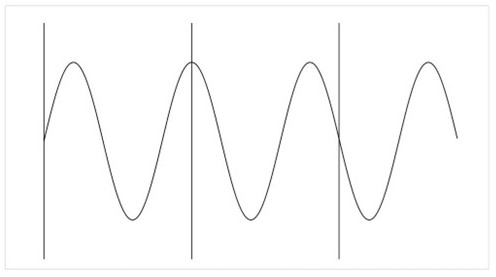
\includegraphics[width=.5\columnwidth]{img/12.jpg}
      \label{sub8}
    }~
    \subfigure[表示波形]{
    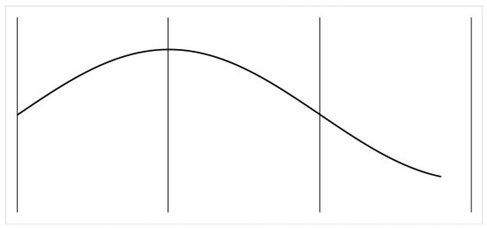
\includegraphics[width=.5\columnwidth]{img/13.jpg}
      \label{sub9}
    }
   \caption{フーリエ級数による近似}
   \label{im8}
   \end{center}
\end{figure}

追加検討1について、実験結果 (1)、実験結果 (2)、実験結果 (3) の実験において、
トリガレベルを正と負のピーク値の間とその間の外に設定した場合の、
ディジタルオシロスコープとアナログオシロスコープについて、
トリガ点は画面左端のままで行っていた。しかし、ディジタルオシロスコープについて、
トリガ点の位置を表示画面の左端以外にも設定できる。そこで、実験1において、
トリガ点を変更させたときの動作の推測とその理由について述べたいと思う。
実験結果 (1) ~ (3) において、トリガレベルを波形のピーク値の間、
トリガ点を横軸方向に移動させたとき、移動させた点から波形が表示される。
また、トリガ点以前の波形を表示させることができると推測できる。
その理由として、ディジタルオシロスコープは原理で述べたように、
ディジタル信号のデータをメモリに保存したのちに、波形を表示するため、
原理図\ref{im1}の演算部において保存されたトリガ点以前のデータを読み込むことによって、
画面にその部分の波形を表示させることができるからである。
一方アナログオシロスコープにおいて、トリガ点を変更することはできない。
なぜなら、ディジタルオシロスコープと違い、波形を保存することができないため、
現時点での波形しか表示できないので、トリガ点以前の現在よりも前の時間の波形を表示させることが
できないからである。従って、アナログオシロスコープにおいて、
トリガレベルを自由に設定できるがトリガポジションを自由に設定できない。
\par
追加検討2について、ディジタルオシロスコープの波形取り込みモードについて、
本実験においてはサンプルモードとアベレージモードにおいての表示波形の変化を観測したが、
アベレージモードは単発信号の波形取り込みができない。
なぜなら、連続波形の取り込みを複数回にわたって行い、波形を平均化して表示波形とするため、
単発信号では波形の表示を1度しかできないため波形の取り込みを1回しかできないからである。
また、アベレージモードの欠点を補うためのモードとして、ハイレゾモードが存在する。
ハイレゾモードとはサンプルモードであるときサンプリング間隔において、
一つのサンプリング間隔にさらに複数のサンプリングをしてそれらのサンプリングを平均し、
波形を表示するといったものになる。

\mysubsection{実験2}
実験結果 (2) において、表\ref{tb2}、 \ref{tb3} より、フーリエ係数$a_n$において、$n$ の値が大きくなるほど、
係数の値が小さくなっていることから、振幅の小さい正弦波の項が足されることによって、
元の波形の垂直成分を再現していることが推測される。
\par
$b_n$ において、$n$ の値が大きくなるほど係数の値が正と負を繰り返すことから、
正と負の振幅を足すことによって波形の垂直成分を定数に近づけて水平成分を平坦にし、
元の波形の水平成分を再現していることが推測される。
\par
実験結果 (3) において
表\ref{tb2}、\ref{tb3}と表\ref{tb4}、\ref{tb5}を比較して、
フーリエ級数 $b_3$, $b_6$, $a_3$, $a_6$ に大きな誤差も見られたが近似波形
図\ref{im8} と図 \ref{im8} は一致している。その理由として、式\eqref{eq5} において、
観測波形の振幅よりも小さい部分とそれよりも大きいとしている部分が相殺し、
近似波形が観測波形に近づいたと推測されるが、数値積分で計算した値の誤差を少なくするために、
標本化の時間間隔をより狭くするようなオシロスコープの設定をするとよい。
\par
フーリエ係数$b_0$について、
式\ref{eq2}を見ると、$b_0$ は観測波形のDC成分を表す。
参考として、フーリエ級数 (数値積分による計算) から$b_0$を引いた値を実験1
実験結果 (6)の時間間隔に対応させて波形を作ると、
入力結合を AC モードとしたときの波形であると推測できる。
(図\ref{im5}) その理由として、 AC モードは波形の正の値を表す面積と負の値を表す面積を等しくし、
観測波形のDC成分を0にするモードであるため、
フーリエ級数におけるDC成分の項$b_0$を0にすることによって、
DC モードの波形を AC モードの波形として描きかえることができるからである。